%\section{}
This chapter introduces \system{K}{n}{}, a \emph{propositional modal logic
language}, semantically determined by an account of necessity and possibility.

A propositional modal language is the well known propositional language augmented
by a collection of \emph{modal operators}. In classical logic, propositions or
sentences are either evaluated to true or false, in any model. Propositional
logic and predicate logic, for instance, do not allow for any further
possibilities. However, in natural language, we often distinguish between
various modalities of truth, such as \emph{necessarily} true, \emph{known to be}
true, \emph{believed to be} true or yet true \emph{in some future}, for example.
Therefore, one may think that classical logics lacks expressivity in this sense. 

Modal logic adds operators to express one or more of these different modes of
truth. Different modalities define different languages. The key concept behind
these operators is that they allow us to reason over relations among contexts or
interpretations, an abstraction that here we think as \emph{possible worlds}.
The purpose of the modal operators is to permit the information that holds at
other worlds to be examined --- but, crucially, only at worlds visible from the
current one via an accessibility relation~\cite{blackburn2002modal}. Then,
evaluation of a modal formula depends on a set of possible worlds and the
accessibility relations defined for these worlds. It is possible to define
several accessibility relations between worlds, and different modal logics are
defined by different relations.

The modal language which is the focus of this work is the extension of the
classical propositional logic that adds the unary operators: $\nec{a}$ and
$\pos{a}$, whose reading are ``is necessary by the agent $a$'' and ``is
possible by the agent $a$'', respectively. This language, known as
\system{K}{n}{}, is characterized by the schema $\nec{a}(\varphi \then \psi) \then
(\nec{a} \varphi \then \nec{a} \psi)$ (axiom \system{K}{}{}), where $a \in \Agents = \{1,
\ldots, n\}$ and $\varphi, \psi$ are well-formed formulae. The addition of other
axioms defines different systems of modal logics and it imposes restrictions on
the class of models where formulae are valid~\cite{chellas:modal_logic}. 

Worlds and their accessibility relations define a structure known as
\emph{Kripke model}. The satisfiability and validity of a formula depend on this
structure. For example, given a Kripke model that contains a set of possible
worlds, a binary relation of accessibility between worlds and a valuation
function that maps in which worlds a proposition symbol holds, we say that a
formula $\nec{}p$ is satisfiable at some world $\st$ of this model, if the
valuation function establishes that $p$ is true at all worlds accessible from
\st.

It is now time to formally define the modal language we will be working with. The
syntax and semantics of \system{K}{n}{} are showed in Sections~\ref{syntax}
and~\ref{semantics}, respectively, and the definitions presented in these two
sections are adaptations from~\cite{journals/jal/NalonD07}.

\section{Syntax}
\label{syntax}

The language of \system{K}{n}{} is equivalent to its set of \emph{well-formed
formulae}, denoted by \wff, which is constructed from a denumerable set of
\emph{propositional symbols} $\Prop = \{p, q, r, \ldots\}$, the negation
symbol $\neg$, the disjunction symbol $\lor$ and the modal connectives
$\nec{a}$, that express the notion of necessity, for each index $a$
in a finite, non-empty fixed set of labels $\Agents = \{1, \ldots, n\}, n
\in \mathbb{N}$.

\begin{definition}
\label{def:wff}
    The set of well-formed formulae, \wff, is the least set such that:
    \begin{enumerate}
        \item $p \in \wff$, for all $p \in \Prop$
            \vspace{.2ex}
        \item if $\varphi, \psi \in \wff$, then so are $\neg \varphi, (\varphi
            \lor \psi)$ and $\nec{a} \varphi$, for each $a \in \Agents$
    \end{enumerate}
\end{definition}

Just as the familiar first-order existential and universal quantifiers are duals
to each other, that is, $\forall x\ \formula \iff \neg \exists x\ \neg \formula$, we have
the dual connectives $\pos{a}$ for necessity, which express possibility, and
they are defined by $\pos{a} \formula \stackrel{def} \neg \nec{a} \neg \formula$, for each
$\agent \in \Agents$. Other logic operators may be used as abbreviations.
In this work, we consider the usual ones:
\begin{itemize}
    \item $\varphi \wedge \psi \stackrel{def} \neg(\neg \varphi \lor \neg \psi)$ (conjuction)
    \item $\varphi \then \psi \stackrel{def} \neg \varphi \lor \psi$ (implication)
    \item $\varphi \iff \psi \stackrel{def} (\varphi \then \psi) \land (\psi \then \varphi)$ (equivalence)
    \item $\textbf{false} \stackrel{def} \varphi \wedge \neg \varphi$ (\emph{falsum})
    \item $ \textbf{true} \stackrel{def} \neg \textbf{false}$ (\emph{verum}) 
\end{itemize}

Parentheses may be omitted if the reading is not ambiguous.  When $n = 1$, we
often omit the index in the modal operators, i.e., we just write $\nec{}
\varphi$ (or `box' \formula) and $\pos{}\varphi$ (or `diamond' \formula), for a
well-formed formula $\varphi$. 

We define as \emph{literal} a propositional symbol $p \in \Prop$ or its negation $\neg
p$, and denote by \Literals~the set of all literals. A \emph{modal literal} is a
formula of the form $\nec{a} l$ or $\pos{a} l$, with $l \in \Literals$ and $a
\in \Agents$.

The following function definitions are based on formulae' syntax. The
\emph{modal depth} of a formula is recursively defined as follows:

\begin{definition}
    We define $mdepth : \wff \longrightarrow \Nat$ to represent the
    maximal number of nesting modal operators in a formula. Inductively:
    \begin{enumerate}
        \item $mdepth(p) = 0$ 
        \item $mdepth(\neg \formula) = mdepth(\formula)$
        \item $mdepth(\formula \lor \psi) = \max\{mdepth(\formula), mdepth(\psi)\}$
        \item $mdepth(\nec{a} \formula) = mdepth(\formula) + 1$
    \end{enumerate}
    With $p \in \Prop$ and $\formula, \psi \in \wff$.
\end{definition}

For instance, if $\formula = \nec{a}\pos{a} p$ then $mdepth(\formula) = 2$ but $mdepth(p) = 0$.

The \emph{modal level} of a formula (or a subformula) is given relative to its position in the
\emph{annotated syntactic tree}.

\begin{definition}
    Let $\Sigma$ be the alphabet $\{1, 2, .\}$ and $\Sigma^*$ the set of all
    finite sequences over $\Sigma$. Denote by $\varepsilon$ the empty sequence.
    We define $\tau : \wff \times \Sigma^* \times \Nat \longrightarrow
    \mathscr{P}(\wff \times \Sigma^* \times \Nat)$ as the partial function
    inductively defined as follows:
    \begin{enumerate}
        \item $\tau(p, \lambda, ml) = \{(p, \lambda, ml)\}$
        \item $\tau(\neg \formula, \lambda, ml) = \{(\neg \formula, \lambda, ml)\} \cup \tau(\formula, \lambda.1, ml)$
        \item $\tau(\nec{a} \formula, \lambda, ml) = \{(\nec{a} \formula, \lambda, ml)\} \cup \tau(\formula, \lambda.1, ml + 1)$
        \item $\tau(\formula \lor \psi, \lambda, ml) = \{(\formula \lor \psi, \lambda, ml)\} \cup \tau(\formula, \lambda.1, ml) \cup \tau(\psi, \lambda.2, ml)$
    \end{enumerate}
    With $p \in \Prop, \lambda \in \Sigma^*, ml \in \Nat$ and $\formula, \psi
    \in \wff$.
\end{definition}

The function $\tau$ applied to $(\formula, \varepsilon, 0)$ returns the
annotated syntactic tree for \formula, where each node is uniquely identified by
a subformula, its position in the tree (or path order) and its modal level. For
instance, $p$ occurs twice in the formula $\nec{a}\pos{a}(p \land \nec{a} p)$,
at the position 1.1.1, with modal level 2, and again at position
1.1.2.1, with modal level 3.

\begin{definition}
    We define $mlevel : \wff \times \wff \times \Sigma^* \longrightarrow \Nat$,
    to represent the maximal number of modal operators in which scope a subformula
    occurs. Let \formula~be a formula and let $\tau(\formula, \varepsilon, 0)$
    be its annotated syntactic tree. If $(\formula', \lambda, ml)\in
    \tau(\formula, \varepsilon, 0)$ then $mlevel(\formula, \formula', \lambda) =
    ml$.
\end{definition}

\section{Semantics}
\label{semantics}

The semantics of \system{K}{n}{} is presented in terms of Kripke structures.

\begin{definition}
    A Kripke model for \Prop~and $\Agents = \{1, \ldots, n\}$ is given by the tuple 
    \begin{equation}
        \Model = (\St, \st_0, R_1, \ldots, R_n, \pi)
    \end{equation}
    where $\St$ is a non-empty set of possible worlds with a distinguinshed world
    $\st_0$, the root of \Model; each $R_a$, $a \in \Agents$, is a binary relation
    on $\St$, that is, $R_a \subseteq \St \times \St$, and $\pi: \St \times \Prop
    \longrightarrow \{false, true\}$ is the valuation function that associates
    to each world $\st \in \St$ a truth-assignment to propositional symbols.
\end{definition}

We denote $R_a \st \upsilon$ to mean that $\upsilon$ is accessible from $\st$ through
the accessibility relation $R_a$, that is $(\st, \upsilon) \in R_a$, and $R^*_a \st
\upsilon$, to mean that $\upsilon$ is reachable from $\st$ through a finite number of
steps, that is, exists a sequence $(\st_1, \ldots, \st_k)$ of worlds such that
$R_a \st_i \st_{i+1}, \forall\ 1 \leq i < k$, where $\st_1 = \st$ and $\st_k =
\upsilon$, with $a \in \Agents$, $\st, \upsilon, \st_i \in W$ and $k \in \Nat$. Note
that $R_a^*$ is the \emph{transitive closure} of $R_a$, the least transitive set
that contains all elements of $R_a$. Here we also make use of the
\emph{transitive and reflexive closure}, denoted by $R_a^+$, the least
transitive and reflexive set that contains all elements of $R_a$.

\emph{Satisfiability} and \emph{validity} of a formula is defined in terms of the \emph{satisfiability relation}.

\begin{definition}
\label{relsat}
    Let $\Model = (\St, \st_0, R_1, \ldots, R_n, \pi)$ be a Kripke model, $\st \in \St$ and $\varphi, \psi \in \wff$. The \emph{satisfiability relation}, denoted by 
    \sat{\Model}{\st}{\varphi}, between a world \st~and a formula $\varphi$,
    is inductively defined by:
    \begin{enumerate}
        \item \sat{\Model}{\st}{p} if, and only if, $\pi(\st, p) = \textbf{true}$, for all $p \in \Prop$;
        \item \sat{\Model}{\st}{\neg\varphi} if, and only if, $
            \langle \Model, \st \rangle \not \models \varphi$;
        \item \sat{\Model}{\st}{\varphi\lor\psi} if, and only if,
            \sat{\Model}{\st}{\varphi} or \sat{\Model}{\st}{\psi}
        \item \sat{\Model}{\st}{\nec{a} \varphi} if, and only if, for all $t\in
            \St$, $(\st, t) \in R_a$ implies  \sat{\Model}{t}{\varphi}
    \end{enumerate}
\end{definition}

Satisfiability is defined with respect to the root of a model. A formula $\varphi
\in \wff$ is said to be \emph{satisfiable} if there exists a Kripke model
$\Model = (\St, \st_0, R_1, \ldots, R_n, \pi)$ such that
\sat{\Model}{\st_0}{\varphi}. In this case we simply write $\Model \models
\formula$ to mean that $\Model$ statisfies \formula~at $\st_0$. A formula is said to be \emph{valid} if it is
satisfiable in all models. We say that a set $\mathcal{F}$ is satisfiable if
every $\formula \in \mathcal{F}$ is satisfiable. Validity of sets is defined
analogously. 

The satisfiability problem for \system{K}{n}{} corresponds to determining the
existence of a model in which a formula is satisfied. This problem is proven to be
PSPACE-complete~\cite{Spaan:coml}.

\begin{example}
    Consider the model illustrated in Figure~\ref{example_semantics}, let's call
    it \Model. Take $\Model = (W, \st_0, R, \pi)$, for $\Prop = \{p\}$ and
    $\Agents = \{1\}$, where 
    \begin{enumerate}
        \item[$(i)$] $W = \{\st_0, \st_1, \st_2\}$
        \item[$(ii)$] $R = \{(\st_1, \st_1), (\st_2, \st_2),
            (\st_0, \st_1), (\st_0, \st_2)\}$
        \item[$(iii)$] $ \pi(\st, p) = 
            \begin{cases} 
                \text{\textbf{true}}    & \quad \text{if } \st = \st_0\\
                \text{\textbf{false}}   & \quad \text{otherwise}
            \end{cases}
                       $
    \end{enumerate}

    Note that both $p$ and $\nec{} \neg p$ are satisfied in \Model. This is a
    rather simple example to illustrate that, even though some sentence
    evaluates to true in the current context, one can see the same sentence
    occurring with the opposite valuation through an accessibility relation.
    This kind of reasoning is not possible in classical logic. Other examples of
    formulae satisfied by this model: $p \land \pos{} \neg p$, $\nec{}\nec{}
    \neg p$ and $\nec{} \nec {} \nec{} \neg p$.
\end{example}

\begin{center}


\begin{figure}[tbh!]
\label{example_semantics}
\begin{center}
%\begin{tabular}{|cc|}
%\hline
%\begin{tikzpicture}[->,rectangle,draw,node distance=1.5cm,
                    %every state/.style={draw=green!30!black!50!,fill=green!10,shape=rectangle,rounded corners,drop shadow,minimum width=3cm}
                   %]
\begin{tikzpicture}[->,circle,draw,node distance=5cm
                   ]

    \node[circle,label=180:$\st_0$,draw,thick](w0){$
        \begin{array}{c}       
            p\\
        \end{array}
    $};
    \node[circle,label=180:$\st_1$,below right of=w0,draw,thick](w1) {$
        \begin{array}{c}       
            \neg p\\
        \end{array}
    $};
    \node[circle,label=0:$\st_2$,below left of=w0,draw,thick](w2) {$
        \begin{array}{c}       
            \neg p\\
        \end{array}
    $};
    \node[circle,label=0:$\st_3$,below left of=w1,draw,thick](w3) {$
        \begin{array}{c}       
             q\\
        \end{array}
    $};
    \path[thick] (w0) edge [below] node {2} (w1)
    (w1) edge [above,loop right] node {1} (w1)
    (w2) edge [above,loop left] node {1} (w2)
    (w0) edge [above,loop] node {1} (w0)
    (w1) edge [above] node {1} (w3)
    (w2) edge [above] node {1} (w3)
    (w0) edge [below] node {2} (w2);

\end{tikzpicture} 
\end{center}

%\hline
%\end{tabular}
    \caption{Example of a Kripke model for \system{K}{n}{}}
\end{figure}
\end{center}



\begin{example}
    \label{ex2}
    (\emph{Tree-like} model) 
    Consider the formula $\formula = \nec{1} (p \then \pos{2} p)$. The
    Figure~\ref{example_models} contains examples of models that satisfy
    \formula. Note that the model from the figure~\ref{example_tree-like} has a
    graphical representation similar to a tree. Finite trees are ubiquitous in
    computer science, they are used to represent knowledge or data from the most
    diverse fields. As trees play such an important role, we will take this
    opportunity to define them, and next, we will show some interesting results
    concerning our modal language.

\begin{figure}
    \begin{subfigure}{.5\textwidth}
          \centering
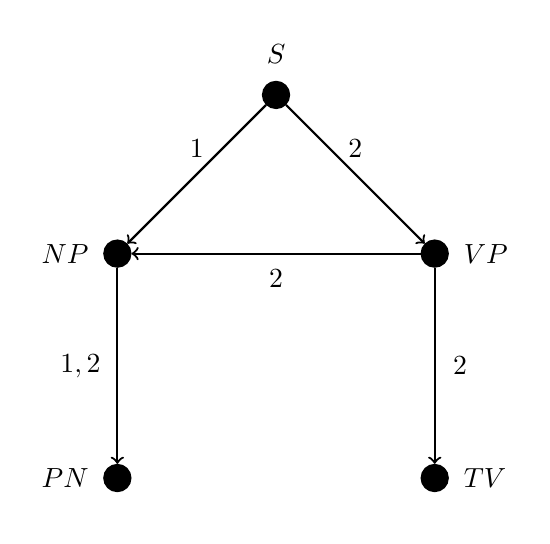
\begin{tikzpicture}[->,circle,draw,node distance=2.85cm,fill=black
                   ]

    \node[circle,label=90:$S$,draw,thick,fill=black](w0){$
    $};
    \node[circle,label=180:$NP$,below left of=w0,draw,thick,fill=black](w1){$
    $};
    \node[circle,label=0:$VP$,below right of=w0,draw,thick,fill=black](w2){$
    $};
    \node[circle,label=180:$PN$,below of=w1,draw,thick,fill=black](w3){$
    $};
    \node[circle,label=0:$TV$,below of=w2, draw,thick,fill=black](w4){$
    $};
    %\node[circle,label=90:$NP'$,below right of=w2, draw,thick,fill=black](w5){$
    %$};
    %\node[circle,label=0:$PN'$,below of=w5,draw,thick,fill=black](w6){$
    %$};
    \path[thick] (w0) edge [above] node {$1$} (w1)
    (w0) edge [above] node {$2$} (w2)
    (w1) edge [left] node {$1,2$} (w3)
    (w2) edge [right] node {$2$} (w4)
    (w2) edge [below] node {$2$} (w1);
    %(w5) edge [below] node {} (w6);

\end{tikzpicture} 
              \caption{Model for phase-structure}
                \label{example_linguistics}
    \end{subfigure}%
    \begin{subfigure}{.5\textwidth}
          \centering
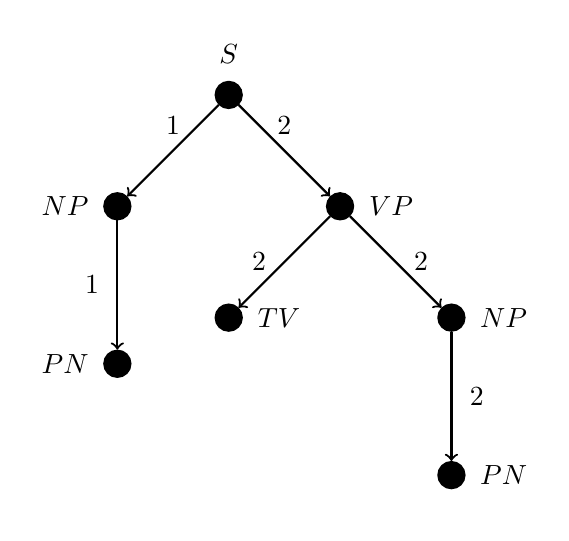
\begin{tikzpicture}[->,circle,draw,node distance=2cm,fill=black
                   ]

    \node[circle,label=90:$S$,draw,thick,fill=black](w0){$
    $};
    \node[circle,label=180:$NP$,below left of=w0,draw,thick,fill=black](w1){$
    $};
    \node[circle,label=0:$VP$,below right of=w0,draw,thick,fill=black](w2){$
    $};
    \node[circle,label=180:$PN$,below of=w1,draw,thick,fill=black](w3){$
    $};
    \node[circle,label=0:$TV$,below left of=w2, draw,thick,fill=black](w4){$
    $};
    \node[circle,label=0:$NP$,below right of=w2, draw,thick,fill=black](w5){$
    $};
    \node[circle,label=0:$PN$,below of=w5,draw,thick,fill=black](w6){$
    $};
    \path[thick] (w0) edge [above] node {$1$} (w1)
    (w0) edge [above] node {$2$} (w2)
    (w1) edge [left] node {$1$} (w3)
    (w2) edge [left] node {$2$} (w4)
    (w2) edge [right] node {$2$} (w5)
    (w5) edge [right] node {$2$} (w6);

\end{tikzpicture} 
              \caption{Tree-like model for phase-structure}
                \label{example_tree-like}
    \end{subfigure}
\end{figure}


 
    By a tree $\mathcal{T}$ we mean a relational structure $(T, S)$ where $T$ is
    a set of nodes and $S$ is a binary relation among these nodes. $T$
    contains a unique~$r_0 \in T$ (called the \emph{root}) such that all
    other nodes in $T$ are reachable from $r_0$, that is, $\forall t \in T$
    we have $S^*r_0 t$, besides that, every element of $T$, distinct from
    $r_0$, has a unique $S$-predecessor, and the transitive and reflexive
    closure $S^+$ is
    acyclic, that is, $\forall t \in T, \neg S^* t t$~\cite{areces2000tree}.

    A \emph{tree model} is a Kripke model $(W, r_0, R, \pi)$, with $\Agents =
    \{1\}$, where $(W, R)$ is a tree and $r_0$ is its root. A \emph{tree-like
    model} for \system{K}{n}{} is a model $(W, r_0, R_1, \ldots, R_n, \pi)$,
    with $\Agents = \{1, \ldots, n\}$, such that $(W, \cup_{i \in \Agents} R_i)$
    is a tree, with $r_0$ as the root.

    In a tree-like model, we can define the \emph{depth} of worlds in $W$.

    \begin{definition}
        Let $\Model = (W, r_0, R_1, \ldots, R_a, \pi)$ be a tree-like model
        for \system{K}{n}{}. We define the $depth: W \longrightarrow \Nat$ of a
        world $\st \in W$, as the length of the path from $r_0$ to $\st$
        through the union of the relations in \Model. We sometimes say $depth$
        of \Model~to mean the largest path from the root to a world in $W$.
    \end{definition}

    \begin{theorem}
        Let $\formula \in \wff$ be a formula and $\Model = (W, \st_0, R_1,
        \ldots, R_n, \pi)$ be a model. Then $\Model \models \formula$ if and only if
        there is a tree-like model $\Model'$ such that $\Model' \models \formula$.
        Moreover, $\Model'$ is finite and its $depth$ is bounded by
        $mdepth(\formula)$.
    \end{theorem}
    \begin{proof}
    \end{proof}

    \begin{theorem}
        Let $\formula, \formula' \in \wff$ and $\Model = (W, \st_0, R_1, \ldots,
        R_n, \pi)$ be a tree-like model such that $\Model \models \formula$. If
        $(\formula', \lambda', ml) \in \tau(\formula, \varepsilon, 0)$ and
        $\formula'$ is satisfied in $\Model$, then there is $\st \in W$, with
        $depth(w) = ml$, such that $\sat{\Model}{\st}{\formula'}$. Moreover,
        the subtree rooted at $w$ has height equals to $mdepth(\formula')$.
    \end{theorem}
    \begin{proof}
    \end{proof}
\end{example}

The \emph{global satisfiability} problem for a modal logic is equivalent to the
satisfiability problem of the logic obtained by adding the universal modality,
$\nec{*}$, to the original language~\cite{goranko1992using}. Let
$\system{K}{n}{*}$ be the logic obtained by adding $\nec{*}$ to \system{K}{n}{}.
Let $\Model = (W, \st_0, R_1, \ldots, R_n, \pi)$ be a tree-like model for
\system{K}{n}{}. A model $\Model^*$ for \system{K}{n}{*} is the pair $(\Model,
R_*)$, where $R_* = W \times W$. A formula $\nec{*} \formula$ is satisfied at
the world $\st \in W$, in the model $\Model^*$, written
\sat{\Model^*}{\st}{\nec{*}\formula}, if, and only if, for all $\st'
\in W$, we have that \sat{\Model^*}{\st'}{\formula}. In this sense, let $\formula
\in \wff$ be a formula, we say that $\formula$ is globally satisfiable in a
model \Model, denoted $\Model \models_G \formula$, if, and only if, $\Model^*
\models \nec{*} \formula$.

\section{Normal Form}

Normal forms can provide elegant and constructive proofs of many standard
results~\cite{fine1975}. This happens because once you translated a set of
formulae into a normal form, you have all your formulae in a specific structure
and possibly less operators to work with, which may implicate into a smaller number
of rules for a proof system. One can even add information into formulae in a
specific normal form. That is the case of the normal form we use in this work.

Formulae in \system{K}{n}{} can be transformed into a layered normal form called
\emph{Separated Normal Form with Modal Levels}, denoted by
\snf{$ml$}~\cite{journals/jal/NalonD07}. A formula in \snf{$ml$} is a
conjunction of \emph{clauses} labelled by the modal level in which they occur.

We write $ml: \formula$ to denote that \formula~occurs at modal level $ml\in
\Nat \cup \{*\}$. By $*: \formula$ we mean that \formula~is true at
all modal levels. Formally, let $\wffml$ denote the set of formulae with
the modal level annotation, $ml : \formula$ such that $ml \in \Nat \cup \{*\}$
and $\formula \in \wff$. Let $\Model^* = (W, \st_0, R_1, \ldots, R_n, R_*, \pi)$
be a model and take $\formula \in \wff$. 

\begin{definition}
Satisfiability of labelled formulae is given by:

\begin{enumerate}
    \item $\Model^* \models ml : \formula$ if, and only if, for all worlds
        $\st \in W$ such that $depth(\st) = ml$, we have
        \sat{\Model^*}{\st}{\formula} 
    \item $\Model^* \models * : \formula$ if, and only if, $\Model^* \models
        \nec{*} \formula$
\end{enumerate}
    
\end{definition}
